\documentclass[11pt,a4paper]{article}
%\usepackage{mathtools,comicsans}
%\usepackage{babel}
\usepackage[utf8]{inputenc}
\usepackage[left=2.5cm,right=2cm, bottom=2cm]{geometry}
\usepackage{amsmath}
\usepackage{amsfonts}
\usepackage{amssymb}
\usepackage{amsfonts}
\usepackage{amsmath}
\usepackage{graphicx}
\usepackage{import}
%\usepackage{subfig}
\usepackage{subcaption}
\usepackage{multirow}
\usepackage{color}
\usepackage{abstract}
\usepackage{float}
\usepackage[toc,page]{appendix}
%\usepackage{url}
\usepackage{hyperref}
\usepackage{todonotes}
\usepackage{tabularx}
%\usepackage{subfigure}
\usepackage{listings}
\DeclareUnicodeCharacter{2212}{-}
\graphicspath{ {./Bilder/} } % Sets path to folder with images/figures


%\renewcaptionname\figureautorefname{Fig.}
\renewcommand{\figureautorefname}{Fig.}
\renewcommand{\figurename}{Fig.}

\newcommand{\overbar}[1]{\mkern 1.5mu\overline{\mkern-1.5mu#1\mkern-1.5mu}\mkern 1.5mu}

%% Algorithm
\usepackage{listings}
\lstset{language=C++}
\lstset{
        mathescape=true,
        morekeywords={if,then,else,return}
        }
\lstset{ 
    captionpos=t,
    tabsize=2
}
\lstset{basicstyle=\ttfamily\footnotesize,breaklines=true}
\renewcommand{\lstlistingname}{Algorithm}% Listing -> Algorithm
\renewcommand{\lstlistlistingname}{List of \lstlistingname s}% List of Listings -> List of Algorithms

\lstset{
    frame=tb, % draw a frame at the top and bottom of the code block
    tabsize=4, % tab space width
    showstringspaces=false, % don't mark spaces in strings
    numbers=left, % display line numbers on the left
    commentstyle=\color{green}, % comment color
    keywordstyle=\color{blue}, % keyword color
    stringstyle=\color{red} % string color
    basicstyle=\footnotesize\ttfamily
}

% double underline
\def\doubleunderline#1{\underline{\underline{#1}}}

\begin{document}
%%%%%%%%% TITLE PAGE %%%%%%%%%
\begin{titlepage}
	\centering
	\begin{center}
	%\includegraphics[width=6cm]{Bilder/IuE-Logo.png}
	\end{center}
	{\scshape\LARGE  Institute for Microelectronics\par}
	\vspace{1cm}
	{\scshape\Large SimFab - Exercise 2\par}
	\vspace{1.5cm}
	\vspace{2cm}
	{\Large\textit{Mario} \textsc{Hiti, 01327428}\par}
	\vspace{1.5cm}
	Submission: May. 23, 2021

\end{titlepage}


\tableofcontents 


\thispagestyle{empty}
\newpage
\setcounter{page}{1}


%%%%%%%%% Begin Document %%%%%%%%%
\section{Requirements}
All vtk files and rendered images can be found in the ./out folder. 
In order to build and run the project the following software packages are required
\begin{itemize}
    \item GCC compiler
    \item Python 3.8.5 or higher
    \item pyvista (for running display.py)
    \item pdflatex (to build the documentation)
\end{itemize}

While ParaView can be used to examine the vtk output files, pyvista is used to render images for the documentation by  invoking a python scriot (display.py)
PyVista still uses the vtk framework as a backend but offers a simple API for rendering files. This way the process of integrating simulation results into the documentation can be automated.

\section{Task 1 - Do you want to Build a Snowman?}
\subsection{Advercting a single sphere}
In this task the combination of multiple shapes and advections is explored.
We start by creating a single sphere and use a constant velociy field to shrink it.

\begin{minipage}{\linewidth}
\begin{lstlisting}[caption=Sphere creation and advection]
// create sphere
auto sphere1 = lsSmartPointer<lsDomain<NumericType, D>>::New(gridDelta);
{

    NumericType origin[3] = {0., 0., 0.};
    NumericType radius = 10.0;
    lsMakeGeometry<NumericType, D>(
        sphere1,
        lsSmartPointer<lsSphere<NumericType, D>>::New(
            origin, 
            radius)
        ).apply(); 
}

lsAdvect<double, D> advectionKernel;
auto constant_vf = lsSmartPointer<ConstantVelocityField>::New(-1);

advectionKernel.insertNextLevelSet(sphere1);
advectionKernel.setVelocityField(constant_vf);
advectionKernel.apply(); 

double advectionSteps = advectionKernel.getNumberOfTimeSteps();
std::cout << Number of Advection steps taken:  << advectionSteps << endl;

>> Number of Advection steps taken: 28
\end{lstlisting}
\end{minipage}

\begin{figure}[h]
    % Rigth image
    \begin{subfigure}{0.45\textwidth}
    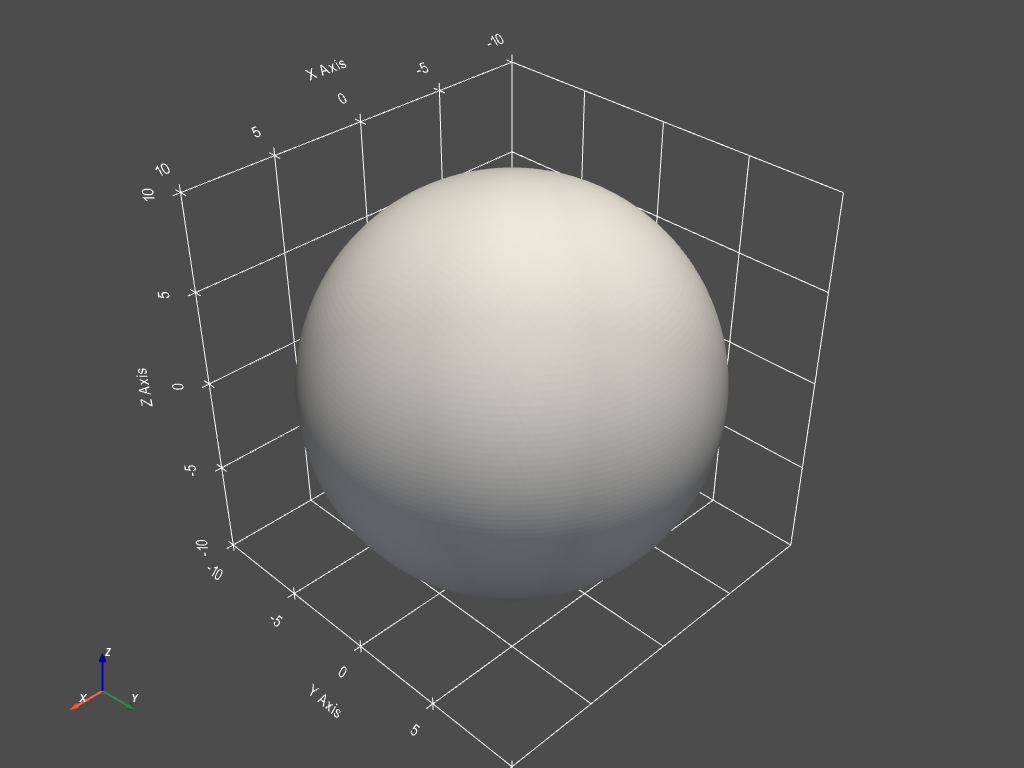
\includegraphics[width=1\linewidth]{res/task1.1_sphere1.png} 
    \caption{The initial sphere}
    %\label{fig:serial-solution}
    
\end{subfigure}
    % left image
    \begin{subfigure}{0.45\textwidth}
    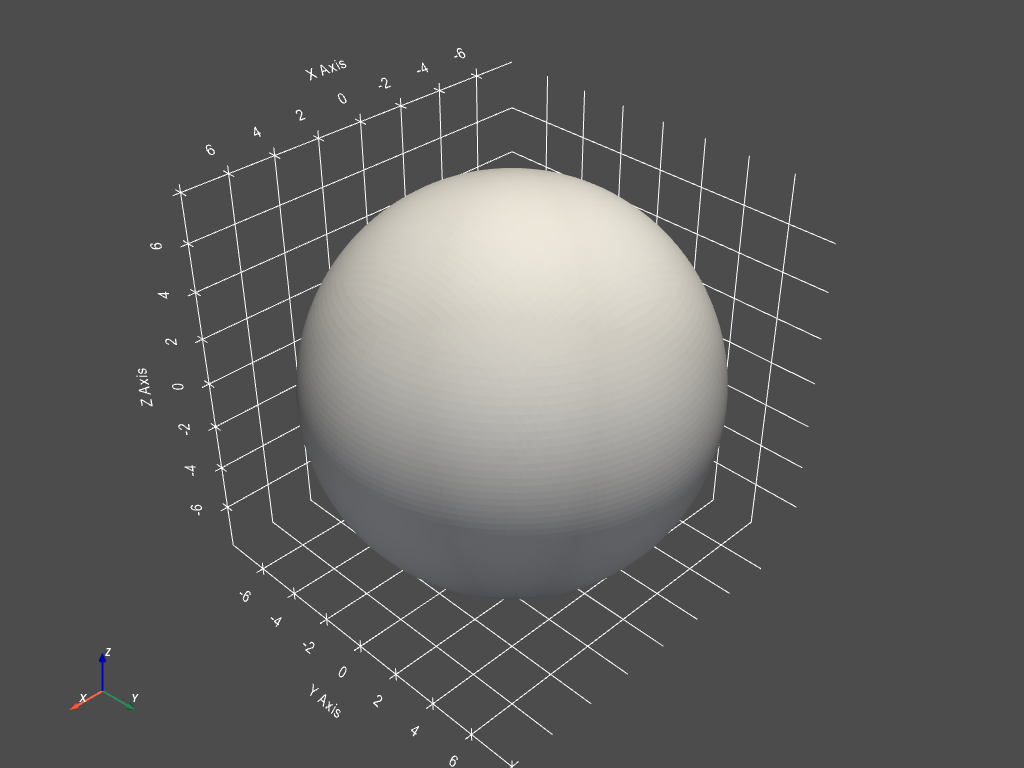
\includegraphics[width=1\linewidth]{res/task1.1_sphere2.png}
    \caption{The sphere after advection}
    %\label{fig:parallel-solution}
\end{subfigure}

\caption{Shrinking a sphere by constant advection. Note that both images use different grid spacings. A positive velocity would result in an expanding sphere (not depicted).}
\label{fig:task1.1_spheres}
\end{figure}

Fig. \ref{fig:task1.1_spheres} shows the sphere with an initial radius = 10 before and after advection. 
The difference in size can be read from the grid axes. A constant velocity field of -2 is used to shrink the object over the period of 1 unit of time. 
Therefore each point has to move 2 units of space towards the center, ths resulting in a new radius = 6.

The results coincide with the expectations and the advection seems to be stable.

\subsection{Combining multiple spheres}
Next multiple spheres are combined to construct a snowman. 
Then a constant velocty field is applied to simulate uniform melting/etching.

\begin{figure}[h]
    % Rigth image
    \begin{subfigure}{0.45\textwidth}
    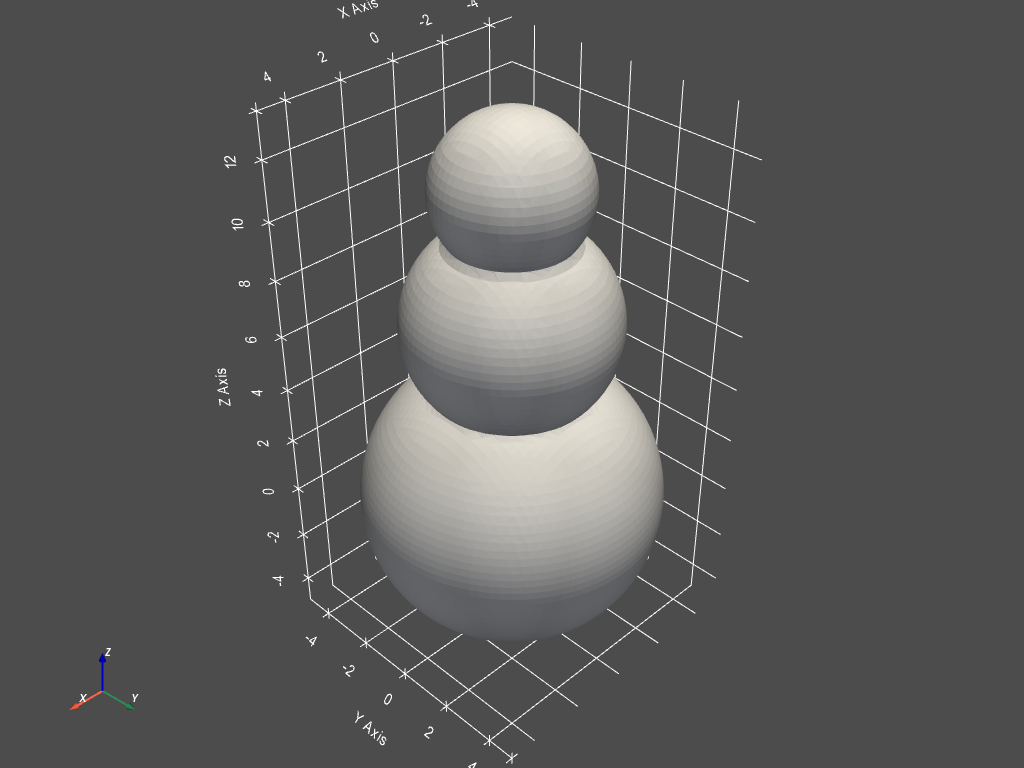
\includegraphics[width=1\linewidth]{res/task1.3_snowman1.png} 
    \caption{The initial snowman}
    
\end{subfigure}
    % left image
    \begin{subfigure}{0.45\textwidth}
    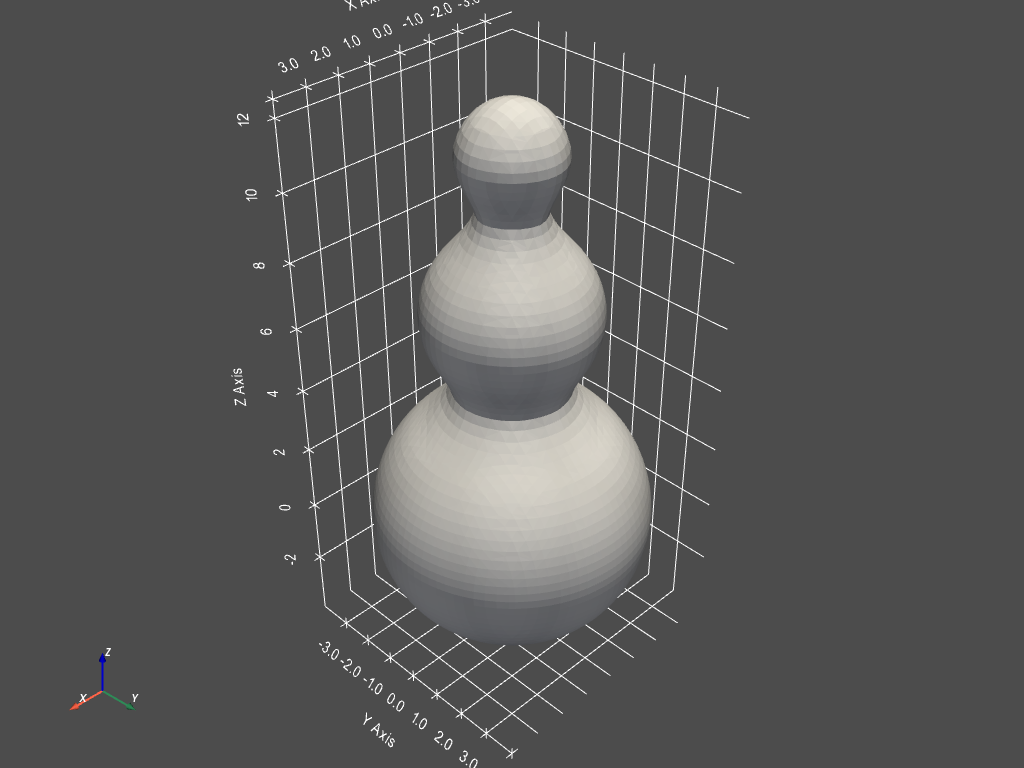
\includegraphics[width=1\linewidth]{res/task1.3_snowman2.png}
    \caption{The snowman after melting}
\end{subfigure}

\caption{Melting a snowman consisting of multiple spheres. Sharp edges where the initial spheres touch become rounded by the advection.}
\end{figure}
\section{Task 2 - Simulating the Bosch process}
The Bosch- or DRIE-etch process is a method to create deep trenches or shappes
with high aspect ratios. Such structures can be used for integrated capacitors or memory devices.

For this task the "drilling" of a circular hole into a substrate is examined.

\subsection{Initial setup}
The Bosch process requires an initial hole in the mask which has to be created by some process as well.
However for this task we assume a perfect cylindrical hole already exists.

We can create the initial layout by stacking a substrate box and a mask box while taking the relative complement with the latter
\begin{figure}[h]
    % Rigth image
    \begin{subfigure}{0.45\textwidth}
    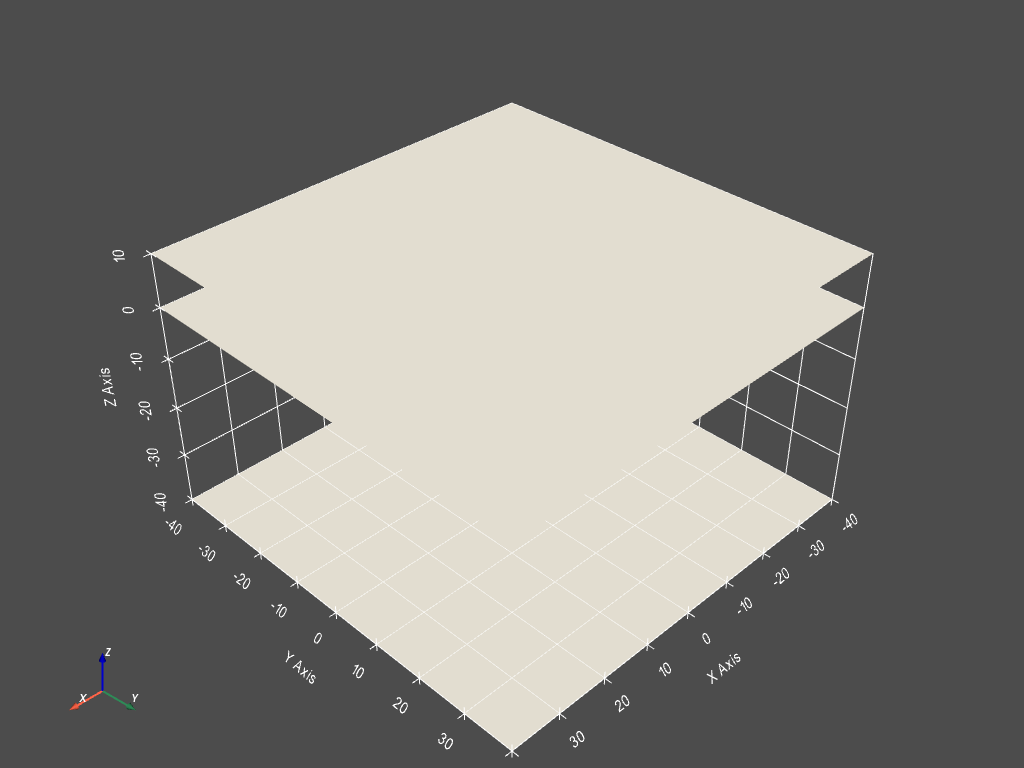
\includegraphics[width=1\linewidth]{res/task2.2_mask.png} 
    \caption{Applying a Mask}
    \label{fig:serial-solution}
    
\end{subfigure}
    % left image
    \begin{subfigure}{0.45\textwidth}
    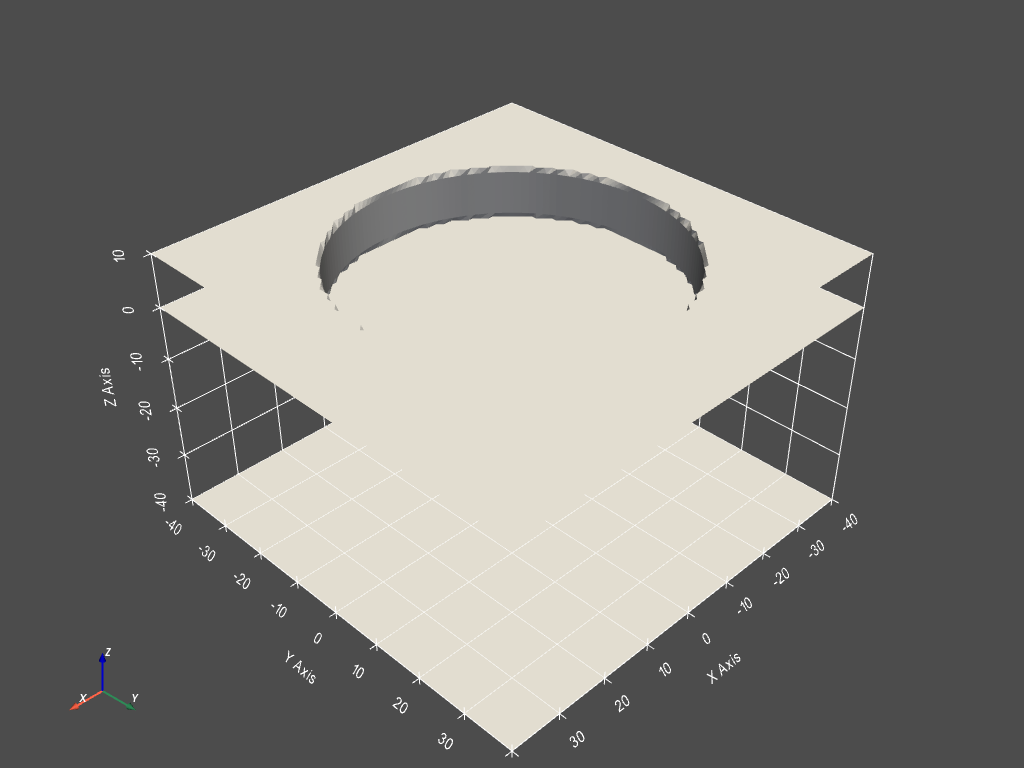
\includegraphics[width=1\linewidth]{res/task2.2_circularHole.png}
    \caption{Cutting a circular hole}
    \label{fig:parallel-solution}
\end{subfigure}

\caption{Creating the initial setup. Mask and substrate appear as planes due to the usage of reflective and infinite boundary conditions}
\label{fig:serial-vs-parallel}
\end{figure}


\subsection{Simulation process}
The process is simulated by performing an initial etch into the substrate followed by 
10 passivation-etch cycles. Substrate etching and passivation is performed uniformly. 
The passivation layer is etched directionally (rate is multiplied by the z-component of the surface normal)

Additionally a randomness factor is introduced to simulate imperfect etching of substrate and and passivation layer.
This is performed by adding a random number from a normal distribution with mean = 0 to the etch rate of all materials as shown in Alg. \ref{cod:etch-field}

\begin{minipage}{\linewidth}
\begin{lstlisting}[caption=etch velocity field, label=cod:etch-field]
double getScalarVelocity(const std::array<double, 3> & /*coordinate*/,
    int material,
    const std::array<double, 3> &normalVector,
    unsigned long /*pointId*/) {
        // if the surface of material 1 is facing upwards, etch it anisotropically
        double vel;
        switch(material)
        {
            case 0:     
                return 0;   // Mask

            case 1:     // substrate
                vel = (-1.)*m_velocity_substrate;
                vel += vel*m_randomNess*distribution(generator);
                return vel;

            default:    // passivation layer
            if(normalVector[2] > 0 )
            {
                vel = (-1)*m_velocity_passivationLayer*std::abs(normalVector[2]);
                vel += vel*m_randomNess*distribution(generator);
                return vel;
            }
            else
            {
                return 0;
            }
        }
    }        
}

\end{lstlisting}
\end{minipage}


Since the mean value of the normal distribution is placed at x=0 both a local increase and decrease in etch rate is possible.
This can be used to model effects such as:
\begin{itemize}
    \item locally increased etch rate caused by particles "breaking off" due mechanical stress such as vibrations
    \item locally decreased etch rate caused by residue being deposited on surface or gas bubbles
    \item crystal granularity if the material is no monocrystal
    \item crystal defects
\end{itemize}


For the purpose of this simulation the deviation from the mean is modelled using a symmetric gauss distribution.

The simulation is set up such that the following parameters are available:
\begin{itemize}
    \item etch time: time in seconds the wafer is submerged in acid
    \item etch velocitry passivation layer: rate at which the passivation material is removed.
    \item etch velocity substrate: rate at which substrate is removed
    \item deposition time: thickness of the passivation layer
    \item steps: number of etch-passivation cycles after the initial etch
    \item randomness: standard deviation of the gauss distribution described above. Random etch rates are calculated relative to the base etch rate. I.e. If the substrate is etched twice as fast the standard deviation is twice as big.
\end{itemize}

\subsection{Results}
The following section shows a selection of possible simulation results with uniform and randomized etch rates after 10 process steps.
The caption below each image shows the simulation parameters which correspond to the listing above.
A quarter of the simulation domain is cut away in order to make the inside of the hole better visible.
Axis units are in nano meters.
\begin{figure}[h]
    % Rigth image
    \begin{subfigure}{0.45\textwidth}
    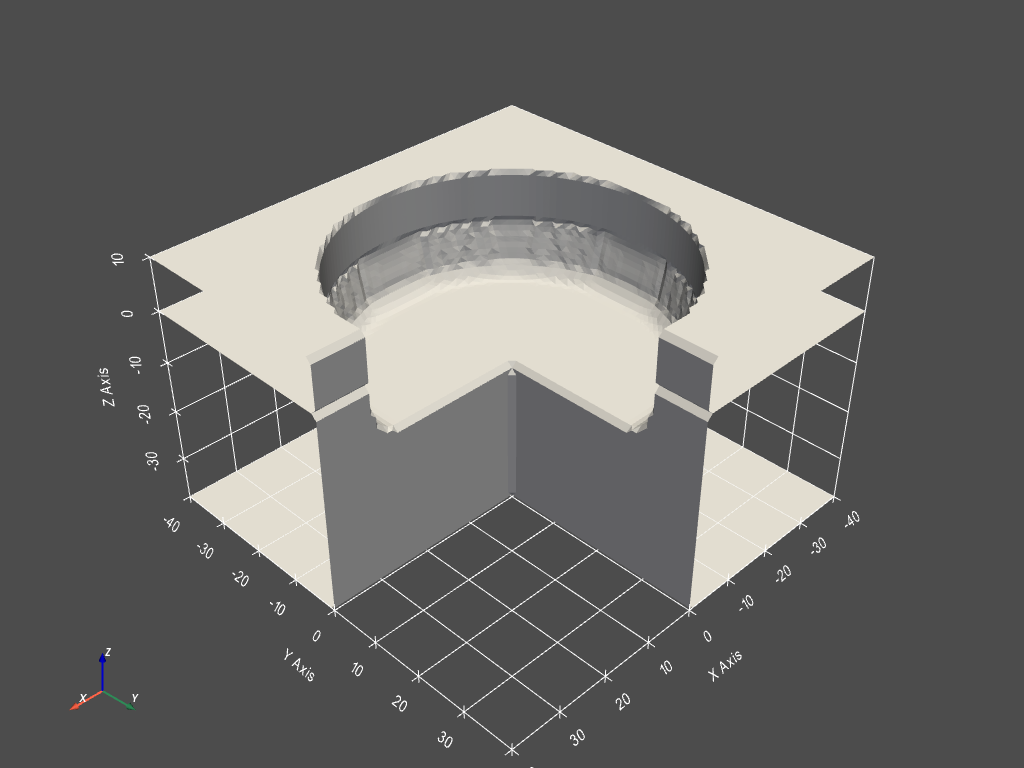
\includegraphics[width=1\linewidth]{res/task2.2_uniformShort.png} 
    \caption{1.5, 1, 0.5, 2.5, 10, 0}
    
\end{subfigure}
    % left image
    \begin{subfigure}{0.45\textwidth}
    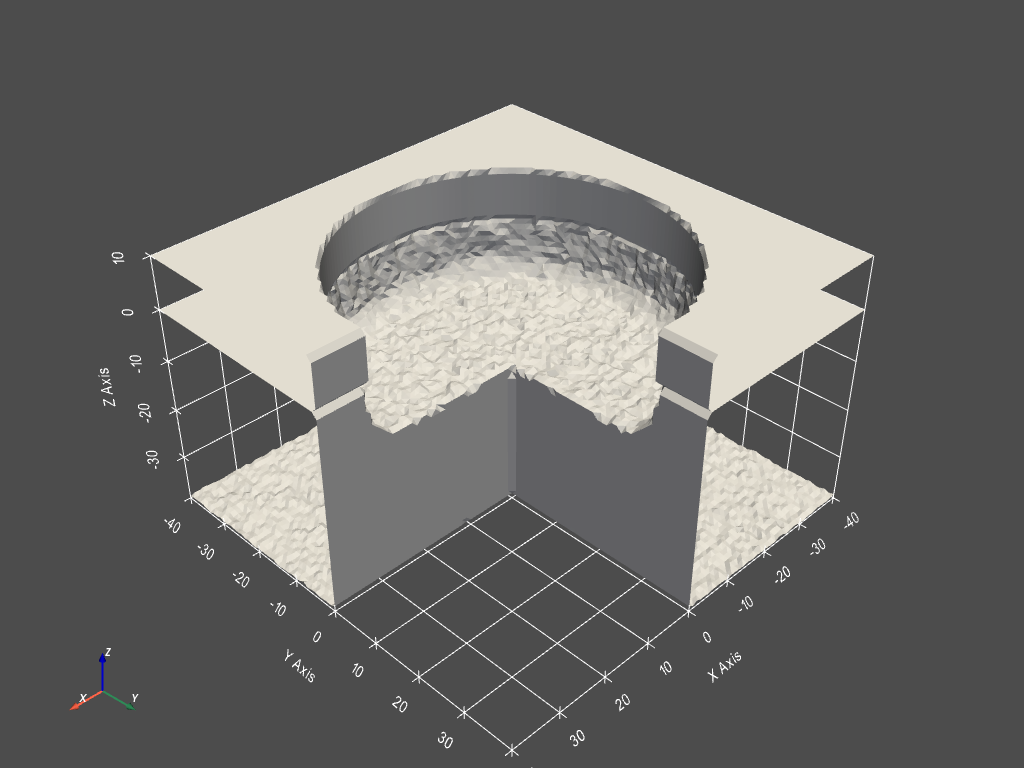
\includegraphics[width=1\linewidth]{res/task2.2_randomShort.png}
    \caption{1.5, 1, 0.5, 2.5, 10, 0}
\end{subfigure}

\caption{Short etchrate. Walls are smoother and single scallops are barely visible}
\end{figure}


\begin{figure}[h]
    % Rigth image
    \begin{subfigure}{0.45\textwidth}
    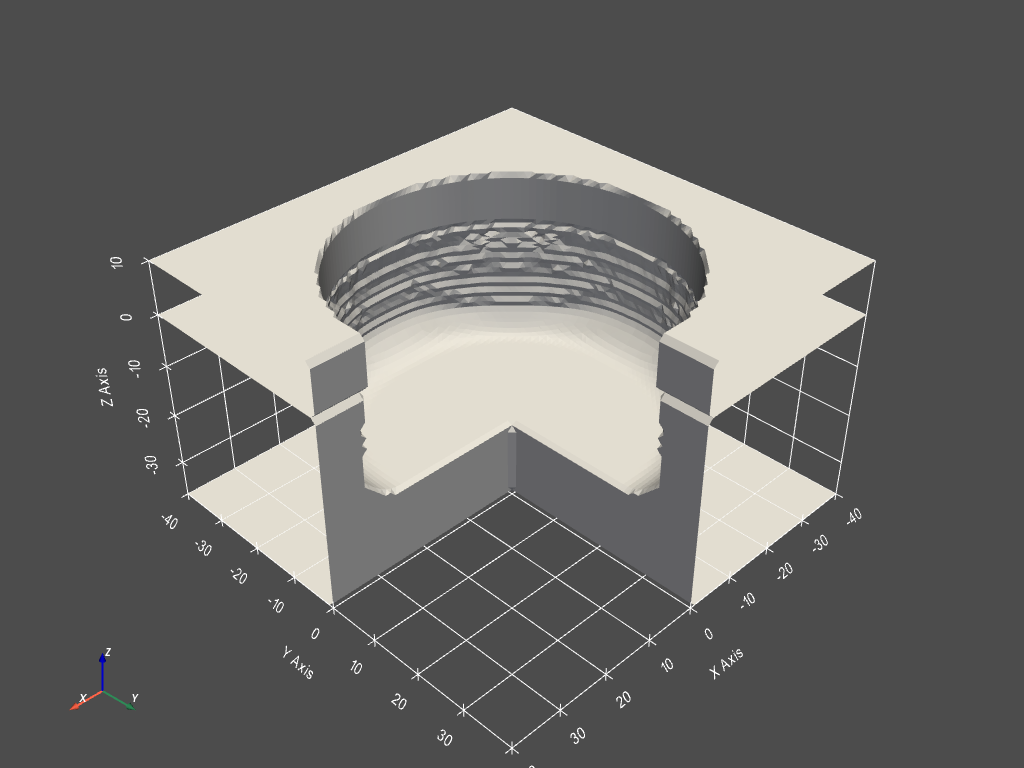
\includegraphics[width=1\linewidth]{res/task2.2_uniformLong.png} 
    \caption{3, 1, 0.25, 2.5, 10, 0}
    
\end{subfigure}
    % left image
    \begin{subfigure}{0.45\textwidth}
    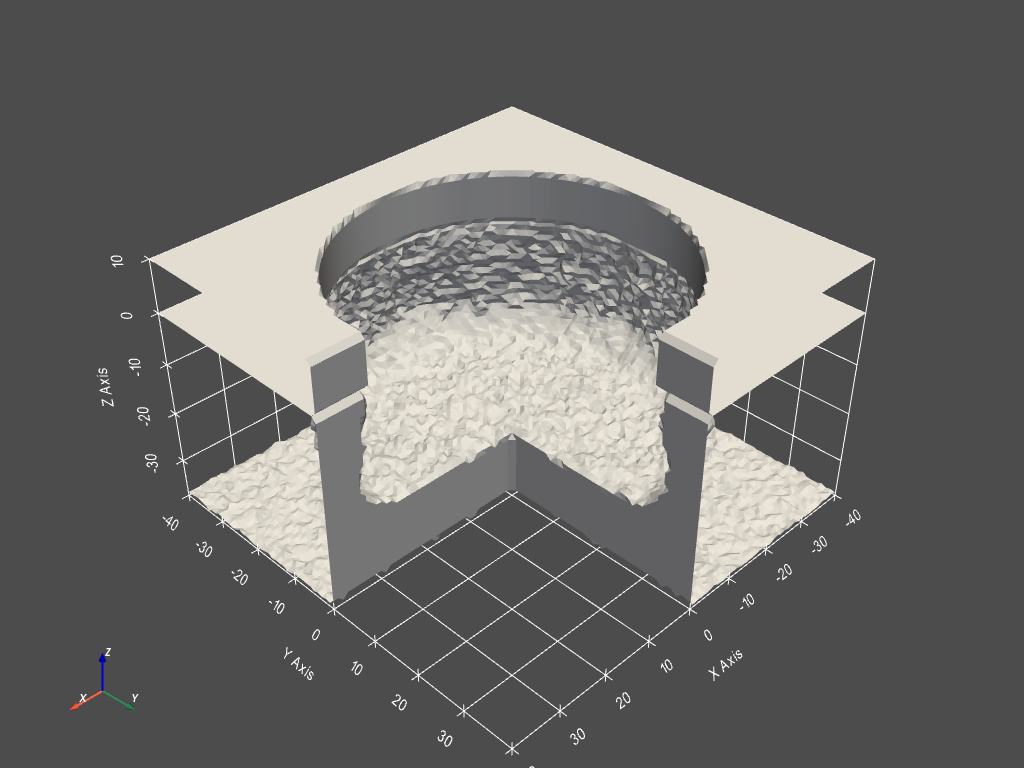
\includegraphics[width=1\linewidth]{res/task2.2_randomLong.png}
    \caption{3, 1, 0.25, 2.5, 10, 0.4}
\end{subfigure}

\caption{Longer etchrate. The hole is significantly deeper but grooves are clearly visible. The randomness blurs "smears" out the grooves but can also create random cavities on the wall}
\end{figure}


\begin{figure}[h]
    % Rigth image
    \begin{subfigure}{0.45\textwidth}
    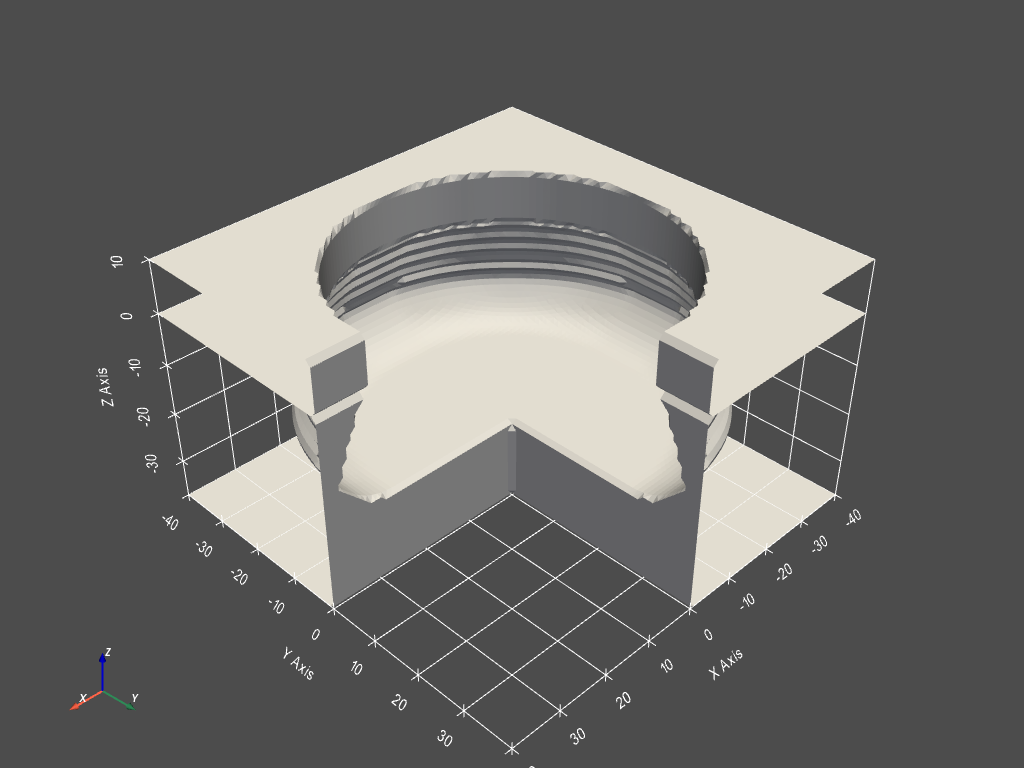
\includegraphics[width=1\linewidth]{res/task2.2_uniformSkewed.png} 
    \caption{2.5, 1, 0.5, 2.5, 10, 0}
    
\end{subfigure}
    % left image
    \begin{subfigure}{0.45\textwidth}
    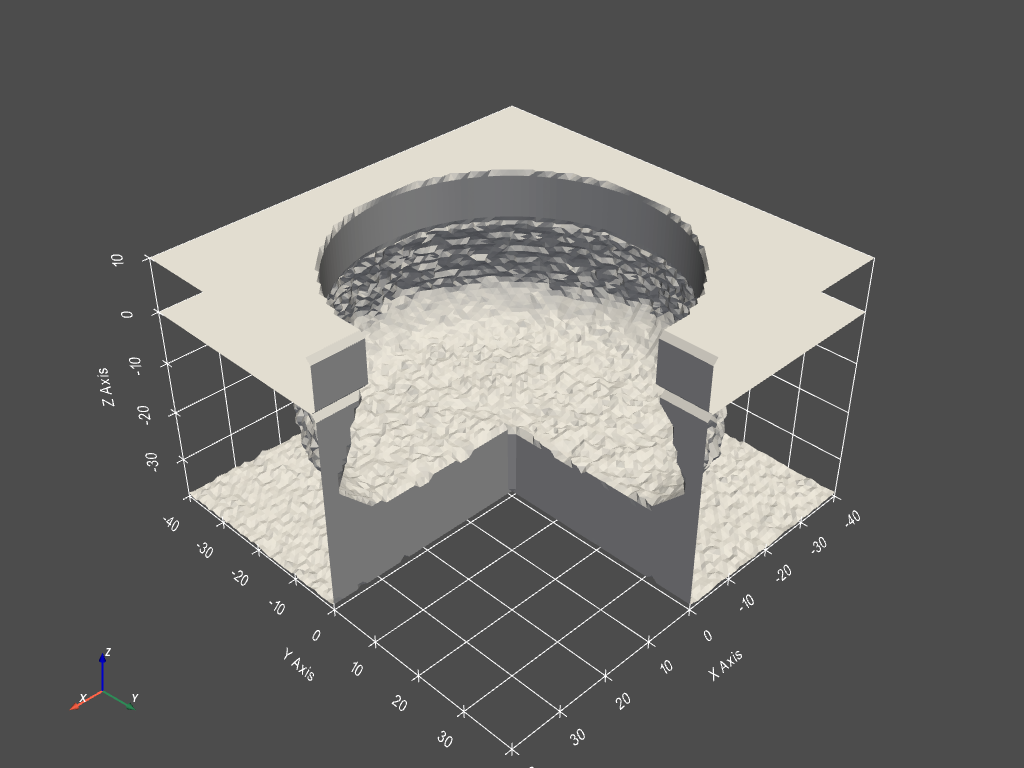
\includegraphics[width=1\linewidth]{res/task2.2_randomSkewed.png}
    \caption{2.5, 1, 0.5, 2.5, 10, 0.4}
\end{subfigure}

\caption{Deep holes but with unbalanced etch and deposition rates. Walls are clearly skewed}
\end{figure}

\subsection{Discussion}
In general it is rather difficult to balance etch- and deposition-rates such that the resulting
wall structure is vertical. This becomes even harder with real materials where rates cannot be arbitrarily set but are defined by the properties of the chosen material.

Depth and wall roughness can best be controlled by adjusting the etch time. While longer etch times can remove more material in each process step the texture of the wall becomes increasingly rough.
Adding randomness to the simulation may smear the edges out by a bit but can also result in bigger random cavities which may have a negative impact on the structural integrity 
if the material is exposed to vibrations or surface tensions during a wet process step.
A rough surface may also be useful for certain applications where a big surface area is needed. 
\begin{figure}[H]
	\centering
	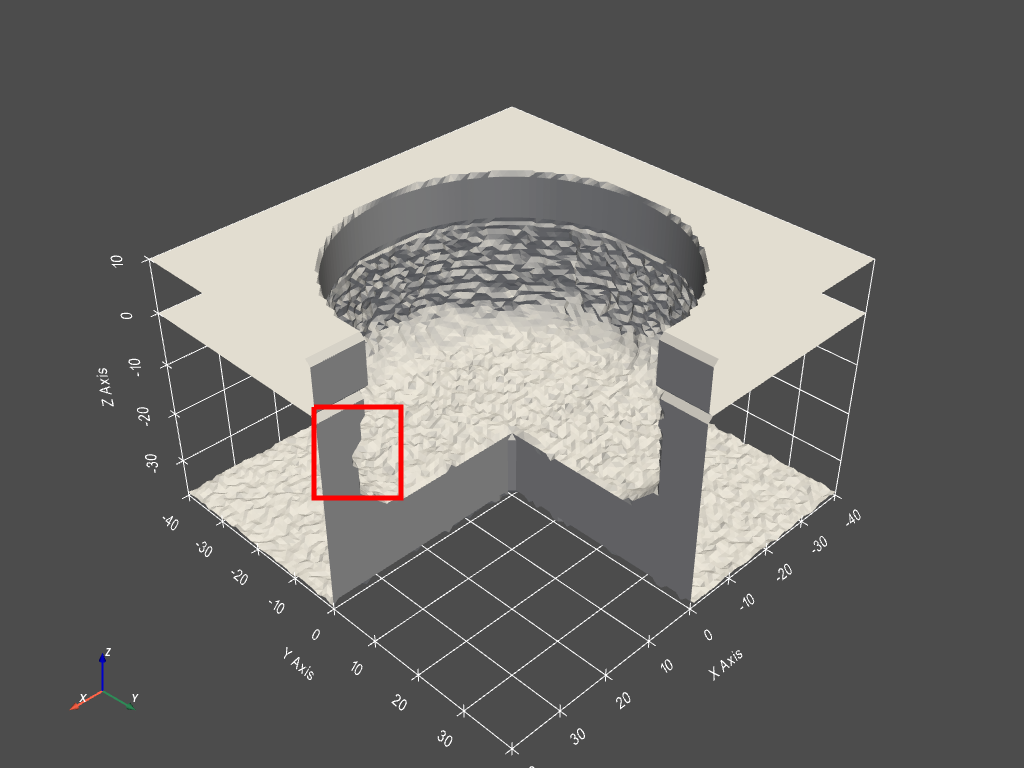
\includegraphics[width=0.75\textwidth]{res/task2.2_cavityBig.png}
	\caption{An example of a bigger random cavity}
\end{figure}

While this process may allow for the creation of structures with high apsect rations it is also very expensive in terms of processing steps.
In addition to etching and deposition further intermediary steps such as cleaning/flushin and quality control are needed (although maybe not between every step)
to achieve good yields. All of these steps are usually performed on different machines.

   
\section{Creating transistor structures}
Unfortunately I did not manage to complete this task since it took me much longer than expected to undcerstand the lsVienna framework.
Therefore I will present only the steps that I did manage to complete and discuss possible further outcomes.

\subsection{Processing steps}
All axis units are in nanometers

\begin{figure}[H]
	\centering
	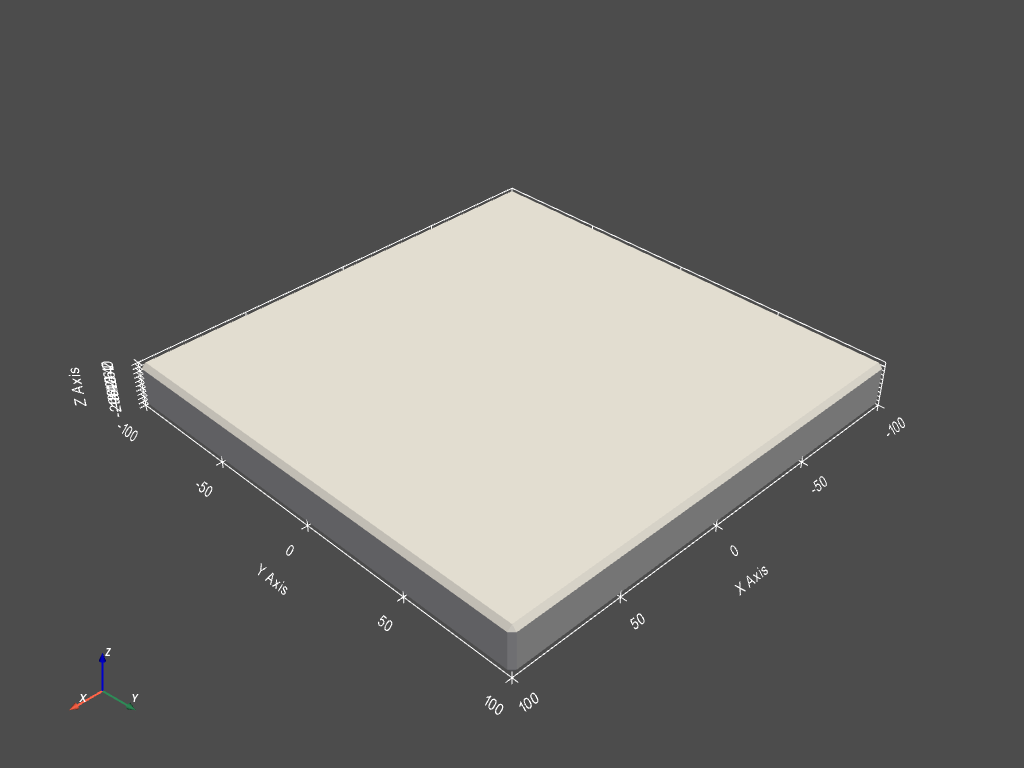
\includegraphics[width=0.75\textwidth]{res/task3_1_oxide_deposition.png}
	\caption{Step 1: Starting with a single 200x200x20nm plate of silicon}
\end{figure}

\begin{figure}[H]
	\centering
	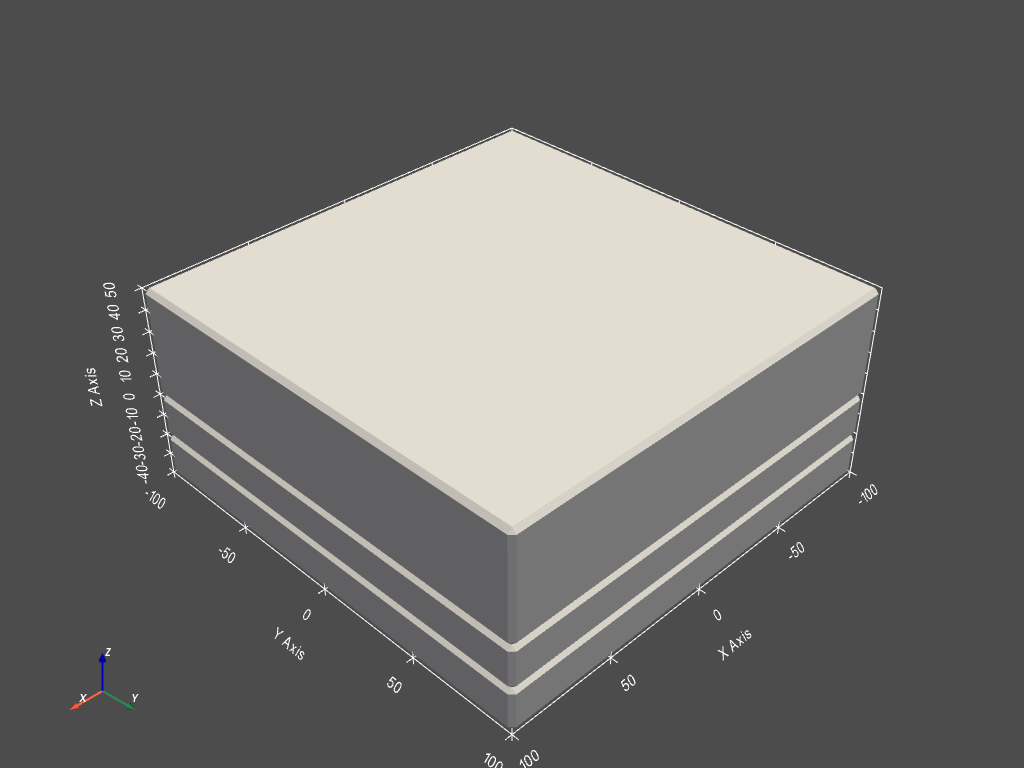
\includegraphics[width=0.75\textwidth]{res/task3_2_silicon_deposition.png}
	\caption{Step 2: Depositing Oxide (middle) and mask (top) on the silicon substrate}
\end{figure}

\begin{figure}[H]
	\centering
	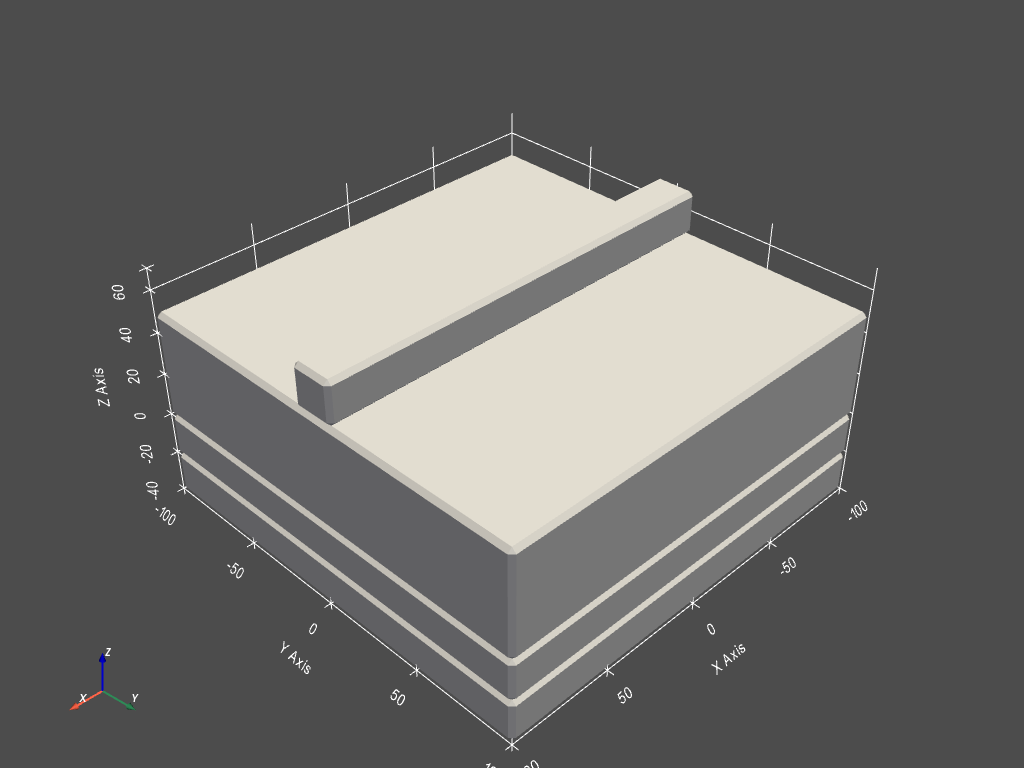
\includegraphics[width=0.75\textwidth]{res/task3_3_mask_cration.png}
	\caption{Step 3: Creating a mask on top of the silicon}
\end{figure}

\begin{figure}[H]
	\centering
	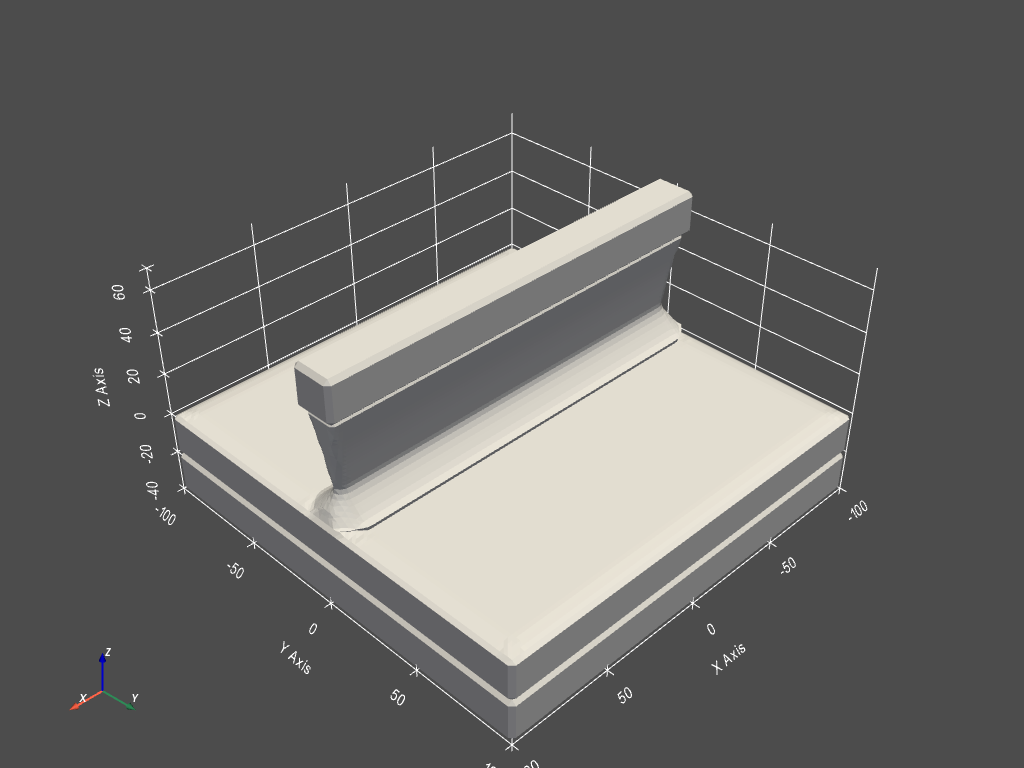
\includegraphics[width=0.75\textwidth]{res/task3_4_fin_creation.png}
	\caption{Step 4: Directionally etching downwards. Etching is not perfectly vertical but is slightly "digging" below the mask.}
    \label{ffig:fin-creation}
\end{figure}

\begin{figure}[H]
	\centering
	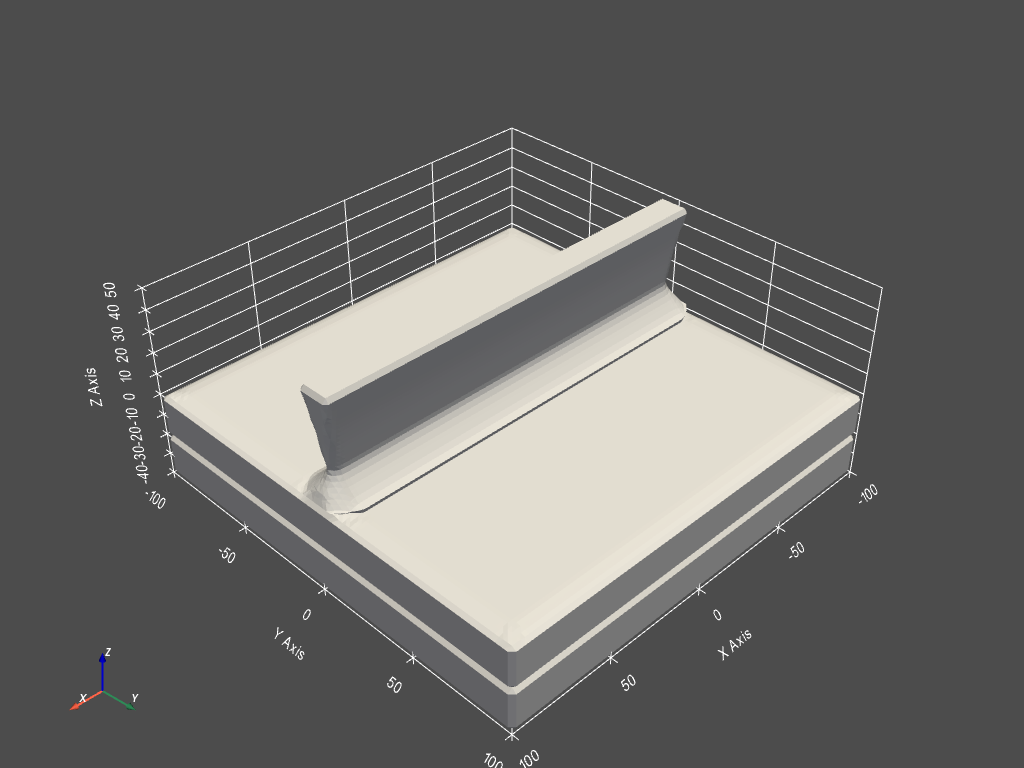
\includegraphics[width=0.75\textwidth]{res/task3_5_maskRemoval.png}
	\caption{Step 5: Mask removal}
\end{figure}


\begin{figure}[H]
	\centering
	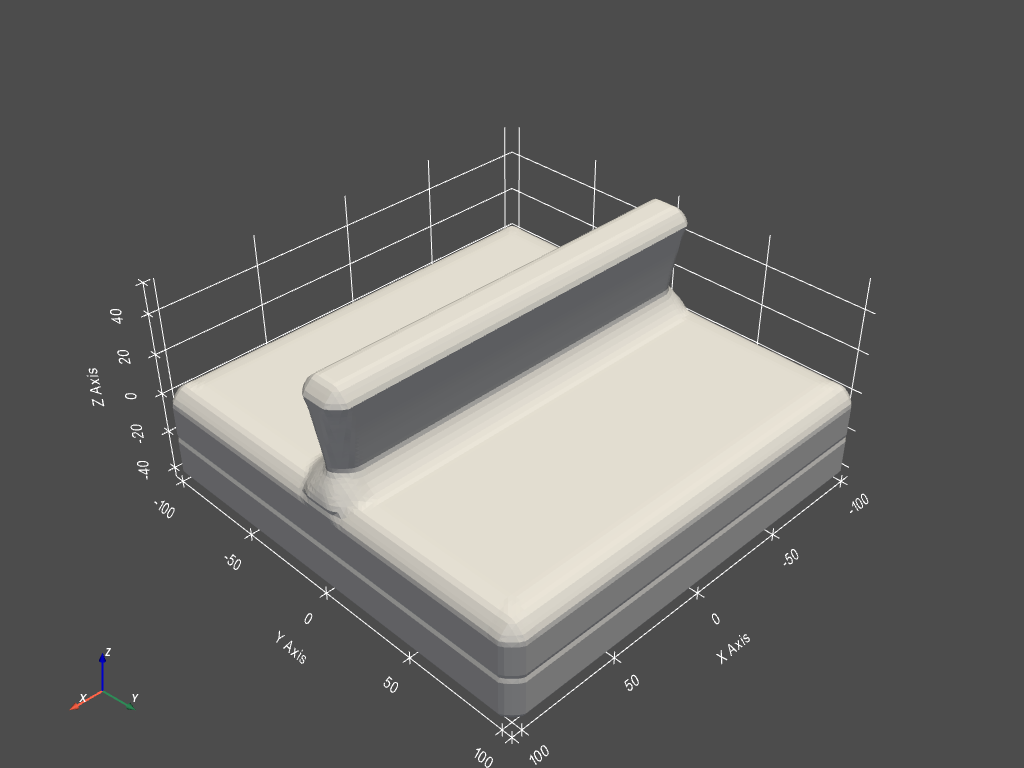
\includegraphics[width=0.75\textwidth]{res/task3_6_spacerDeposition.png}
	\caption{Step 6: Uniform spacer deposition}
    \label{fig:spacer-deposition}
\end{figure}


\begin{figure}[H]
	\centering
	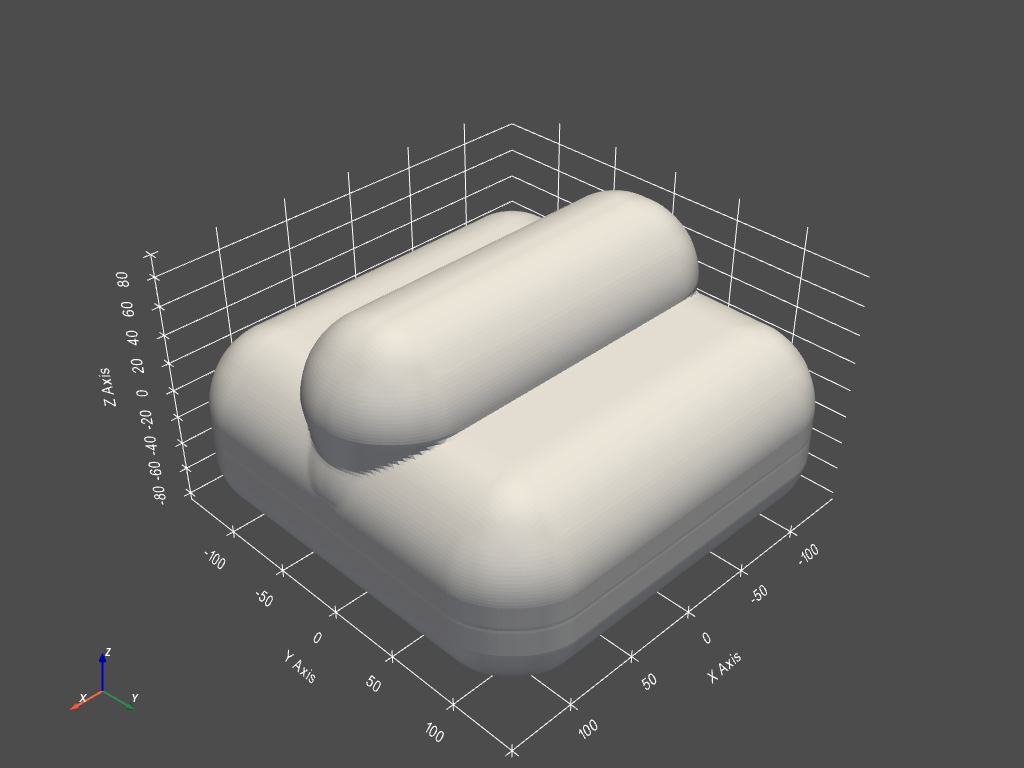
\includegraphics[width=0.75\textwidth]{res/task3_7_gateDeposition.png}
	\caption{Step 7: Gate deposition}
    \label{fig:gate-deposition}
\end{figure}

One can see that something is not working in step 7 (Fig. \ref{fig:gate-deposition}).
I suspect that the reason behind this is the absence of properly defined boundary conditions or I am not defining materials correctly.
Unfortunately at this step I have run out of time to fix issues.

However if that problem would be fixed creating the gate structure should be analog to creating the fin structure.

As seen in \ref{ffig:fin-creation} the etching process is not perfectly straigh but a slight anisotropy is rpesent.
This results in a smaller cross section near the base of the fin. If we would continue to etch then the fin would just break off.

If a positive isotropic component where to be introduced than etched structures would have walls that are skewed outwards instead of inwards (as shown in Fig. \ref{ffig:fin-creation}).





   
\end{document}